% Präambel
\documentclass[12pt,a4paper,oneside, 
liststotoc, 					% Tabellen- und Abbildungsverzeichnis ins Inhaltsverzeichnis
bibtotoc,						% Literaturverzeichnis ins Inhaltsverzeichnis aufnehmen
titlepage, 						% Titlepage-Umgebung statt \maketitle
headsepline, 					% horizontale Linie unter Kolumnentitel
%abstracton,					% Überschrift beim Abstract einschalten, Abstract muss dazu in {abstract}-Umgebung stehen
%DIV11,							% auskommentieren, um den Seitenspiegel zu vergrößern
BCOR6mm,						% Bindekorrektur, die den Seitenspiegel um 6mm nach rechts verschiebt,
]{scrreprt}			
\usepackage{ucs} 				% Dokument in utf8-Codierung schreiben und speichern
\usepackage[utf8x]{inputenc} 	% ermöglicht die direkte Eingabe von Umlauten
\usepackage[ngerman]{babel} 	% deutsche Trennungsregeln und Übersetzung der festcodierten Überschriften
\usepackage[T1]{fontenc} 		% Ausgabe aller zeichen in einer T1-Codierung (wichtig für die Ausgabe von Umlauten!)
\usepackage{graphicx}  			% Einbinden von Grafiken erlauben
\usepackage{amsmath}
\usepackage{amsfonts}
\usepackage{amssymb}
\usepackage{mathpazo} 			% Einstellung der verwendeten Schriftarten
\usepackage{textcomp} 			% zum Einsatz von Eurozeichen u. a. Symbolen
\usepackage{listings}			% Datstellung von Quellcode mit den Umgebungen {lstlisting}, \lstinline und \lstinputlisting
\usepackage{xcolor} 			% einfache Verwendung von Farben in nahezu allen Farbmodellen
\usepackage[intoc]{nomencl}  	% zur Erstellung des Abkürzungsberzeichnisses
\usepackage{fancyhdr}			% Zusatzpaket zur Gestaltung von Fuß und Kopfzeilen
\usepackage{titleref}			% Zum referenzieren mit Überschrift
\usepackage{varwidth}			%alighn asci figure
\usepackage{chngcntr}			% Tabellen- und Abbildungsverzeichnis als fortlaufende Nummer
\usepackage{hyperref}
\usepackage[justification=centering]{caption} % Bild unterschrift mittig ausrichten
\usepackage{nameref}
\counterwithout{figure}{chapter}
\counterwithout{table}{chapter}
\usepackage{url}
\usepackage{float}
\usepackage[framemethod=tikz]{mdframed}
\usetikzlibrary{calc}
\usepackage{tikz}
\usepackage[tikz]{bclogo}
\usetikzlibrary{shapes,arrows}


% Define block styles
\tikzstyle{decision} = [diamond, draw, fill=blue!20, 
    text width=4.5em, text badly centered, node distance=3cm, inner sep=0pt]
\tikzstyle{block} = [rectangle, draw, fill=blue!20, 
    text width=5em, text centered, rounded corners, minimum height=4em, node distance=3cm]
\tikzstyle{line} = [draw, -latex']
\tikzstyle{cloud} = [draw, ellipse,fill=red!20, node distance=2cm,
    minimum height=2em]



\tikzset{
	lampsymbol/.style={%
		,scale=2,overlay}}
	
\newmdenv[nobreak,middlelinewidth=.8pt,
frametitlefont=\bfseries,
leftmargin=.3cm,rightmargin=.3cm, innerleftmargin=2cm,
skipabove=\topsep,skipbelow=\topsep,
singleextra={\path let \p1=(P), \p2=(O) in ($(\x2,0)+0.5*(2,\y1)$) node[ lampsymbol, rotate=20] {\bclampe};
	\draw[line width=.8pt,white,] ($(O|-P)+(.2cm,0)$) -- ($(P)-(.2cm,0)$); 
	\draw[line width=.8pt,white,] ($(O)+(.2cm,0)$) -- ($(P|-O)-(.2cm,0)$);
},%
]{lamp}

%\usepackage[none]{hyphenat} %deaktiviert Silbentrennung
%\usepackage{showframe}% zum Anzeigen des Seitenlayouts
%Abstand vor Chapter
\renewcommand*\chapterheadstartvskip{\vspace*{-\topskip}}
\renewcommand*\chapterheadendvskip{%
  \vspace*{1\baselineskip plus .1\baselineskip minus .167\baselineskip}}


\setlength\abovedisplayshortskip{0pt}
\setlength\belowdisplayshortskip{0pt}
\setlength\abovedisplayskip{20pt}
\setlength\belowdisplayskip{20pt}

% -----------------------------------------------------------------------------------------------------------------
% Zum Aktualisieren des Abkürzungsverzeichnisses bitte auf der Kommandozeile folgenden Befehl aufrufen :
%  makeindex Bachelorarbeit.nlo -s nomencl.ist -o Bachelorarbeit.nls
% -----------------------------------------------------------------------------------------------------------------

% Hier die persönlichen Daten eingeben:

\newcommand{\titel}{Dienstplan}
\newcommand{\untertitel}{Benutzerhandbuch für das Dienstplan-Portal
 
\url{https://dlrgdienstplan.de/}}
\newcommand{\autor}{Philippe Käufer}
\newcommand{\version}{2022.1}

\newcommand{\ovretextfalt}{%
Herausgeber: \\
Philippe Käufer\\
Lembergstraße 11\\
70825 Korntal\\
dienstplan@philhil.de \\
\url{https://dlrgdienstplan.de/impressum}
}

% Abkürzungen
\newcommand{\ua}{\mbox{u.\,a.\ }}
\newcommand{\zB}{\mbox{z.B.\ }}
\newcommand{\bs}{$\backslash$}
\newcommand{\Csharp}{C\#}

\renewcommand{\nomname}{Abkürzungsverzeichnis}
\makenomenclature 

% -------------------------------------------------------------------------------------------
% Definition der Kopf- und Fußzeilen
\lhead{}								% Kopf links
\chead{}								% Kopf mitte
\rhead{\sffamily{\titel}}				% Kopf rechts
\lfoot{}								% Fuß links
\cfoot{\sffamily{\thepage}}				% Fuß mitte
\rfoot{\sffamily{\autor}}				% Fuß rechts
\renewcommand{\headrulewidth}{0.4pt}	% Liniendicke Kopf
\renewcommand{\footrulewidth}{0.4pt}	% Liniendicke Fuß

\makenomenclature						% Abkürzungsverzeichnis erstellen

% alle Abkürzungen, die in der Bachelorarbeit verwendet werden

\nomenclature{CI}{Corporate Identity }

\nomenclature{Dienst}{Eine Freiwilligenarbeit für eine definierte Zeit. Meist im Wasserrettungsdienst oder Freibad. Der Dienst definiert wann und eventuell wie lange und wo die Freiwilligearbeit zu tätigen ist. Ein Dienst enthält eine oder mehrere zu besetzende Positionen.}

\nomenclature{Gliederung}{Repräsentiert eine hierarchische Organisations-Einheiten (z.B. Bundesverband, Landesverband, Bezirke oder Ortsgruppe). Typischerweise wird in der Softwareentwicklung equivalent die Begriffe Mandant oder Client verwendet.}

\nomenclature{GUI}{Grafische Benutzeroberfläche oder auch grafische Benutzerschnittstelle (graphical user interface) }

\nomenclature{ORM}{Objektrelationale Abbildung (object-relational mapping) }

\nomenclature{Position}{Eine zu besetzende Freiwillgearbeit mit vordefinierten vorraussetzungen wie Wissen und Können (Qualifikation). Eine Position ist immer einem Dienst zugeordnet.}

\nomenclature{Qualifikation}{Ein definiertes Wissen und Können welches meist durch Besuchen von Lehrgängen und Fortbildungen erlangt werden kann.}

\nomenclature{RWD}{(Responsive Web Design) Die Größe und Auflösung der Displays auf Laptops, Desktop-PCs, Tablets und Smartphones können erheblich variieren. Aus diesem Grund ist das Erscheinungsbild und die Bedienung einer Website stark abhängig vom Endgerät. Aufgrund dessen werden Webseiten mit einem Design ausgestattet welches sich auf die unterschiedlichen Anforderungen der Endgeräte anpassen. \cite{Responsive_Webdesign}
}				% Datei mit Abkürzungen laden


% -------------------------------------------------------------------------------------------
%                     Beginn des Dokumenteninhalts
% -------------------------------------------------------------------------------------------
\begin{document}
\setcounter{secnumdepth}{2}					% Nummerierungstiefe fürs Inhaltsverzeichnis
\setcounter{tocdepth}{2}
\sffamily									% für die Titelei serifenlose Schrift verwenden

% ------------------------------ Titelei -----------------------------------------------------

\thispagestyle{plain}
\begin{titlepage}
\enlargethispage{4.0cm}
%\sffamily 								% Serifenlose Grundschrift für die Titelseite einstellen

\begin{tikzpicture}[remember picture,overlay]%
	\node (nw) at (current page.north west) {};
	\node [xshift=0.2\paperwidth] (ne) at (nw) {};
	\node (sw) at (current page.south west) {};
	\node [xshift=0.2\paperwidth] (se) at (sw) {};

	% Farbiges Feld links
	%\filldraw[fill=yellow!90!black, draw=yellow!90!black] (nw) rectangle (se);
	\node (bard) at (nw) [anchor=north west,fill=red,minimum width=0.2\paperwidth,minimum height=\paperheight] {};

	% DLRG Wortmarke
	\node [anchor=north west,yshift=-2.5cm] at (bard.north west) {%
		\includegraphics[width=0.185\paperwidth]{Bilder/DLRG-GELB.png}%
	};
	
	
	% Textfeld TOP
	\node (ovretext) [anchor=north west,align=left,yshift=-2.5cm,xshift=12pt,font=\sffamily] at (bard.north east) {%
		\ovretextfalt%
	};

	% Grafik mitte
	\node [anchor=north west,yshift=-2cm] at (ovretext.center) {%
		\includegraphics[height=8cm]{Bilder/DienstplanDLRG_Kalender.png}%
	};

	% Titel
	\node (titel) [anchor=north west,yshift=-7cm+-2cm,align=left,text width=0.6\paperwidth,font=\LARGE\sffamily] 
		at (ovretext.south west) {%
		\textbf{\titel}%
	};

	% Untertitel
	\node (undertitel) [anchor=north west,yshift=-6pt,align=left,text width=0.6\paperwidth,font=\large\sffamily] 
		at (titel.south west) {%
		\untertitel%
	};

	% Author
	\node (forfattare) [anchor=south west,yshift=4cm,xshift=12pt,align=left,font=\sffamily] 
		at (bard.south east) {%
		Authoren und Mitwirkende: \autor%
	};
	
	
	% Version
	\node (forfattare) [anchor=south west,yshift=3cm,xshift=12pt,align=left,font=\sffamily] 
		at (bard.south east) {%
		Version: \version%
	};
	
	% Logo unten rechts
	%\node (logo) [anchor=south east,xshift=-18pt,yshift=18pt] at (current page.south east) {%
	%	\includegraphics[width=0.2\paperwidth]{Bilder/Logo-B-Schwarz.png}%
	%};
\end{tikzpicture}

\end{titlepage}
\rmfamily 				% erzeugt die Titelseite
\pagenumbering{Roman}						% große, römische Seitenzahlen für Titelei
\chapter*{Abstract} %*-Variante sorgt dafür, das Abstract nicht im Inhaltsverzeichnis auftaucht

Das DLRG Dienstplan-Portal dient zur Vereinfachung der Planung von Diensten im Ehrenamt. Der Prozess des Ausschreibens zu besetzender Dienste, der Helfer-Meldung wie auch jährlichen Statistik werden mit diesem Portal abgebildet.

\vspace*{5mm} \noindent Ziel ist es den ehrenamtlichen Helferinnen und Helfern eine Übersicht des aktuellsten Standes der Diensteinteilung wie auch selber Einflussmöglichkeiten zu geben. Die Helfer können selbst  partizipieren und Dienstwünsche direkt einreichen. 

\vspace*{5mm} \noindent Das Benutzerhandbuch für das DLRG Dienstplan-Portal hat den Zweck, eine Übersicht der Funktionen aus Sicht eines Anwenders zu geben. In diesem Dokument sind die einzelnen Funktionen und Prozesse im Detail erläutert und mit Grafiken als auch Beispielen aus der Anwendung verdeutlicht. \\
Genderhinweis: Aus Gründen der besseren Lesbarkeit wird auf eine geschlechtsneutrale Differenzierung verzichtet. Entsprechende Begriffe gelten im Sinne der Gleichbehandlung grundsätzlich für beide Geschlechter. Die verkürzte Sprachform beinhaltet keinerlei Wertung.   				% Einbinden des Abstracts

\tableofcontents							% Erzeugen des Inhalsverzeichnisses
\printnomenclature[2.0cm]					% Erzeugen des Abkürzungsverzeichnisses
\listoffigures 								% Erzeugen des Abbildungsverzeichnisses 
%\listoftables 								% Erzeugen des Tabellenverzeichnisses
\pagebreak


% --------------------------------------------------------------------------------------------
%                    Inhalt der Bachelorarbeit
%---------------------------------------------------------------------------------------------
\pagenumbering{arabic}						% arabische Seitenzahlen für den Hauptteil
\pagestyle{fancy}					
\rmfamily
\noindent

\chapter{Einführung}
\label{cha:Einleitung}


\section{Quellcode und Lizenz}
\label{sec:licens_code}
Dieses Projekt steht unter der MIT Lizenz.

\vspace*{5mm} \noindent Hiermit wird unentgeltlich jeder Person, die eine Kopie der Software und der zugehörigen Dokumentationen (die \glqq Software \grqq) erhält, die Erlaubnis erteilt, sie uneingeschränkt zu nutzen, inklusive und ohne Ausnahme mit dem Recht, sie zu verwenden, zu kopieren, zu verändern, zusammenzufügen, zu veröffentlichen, zu verbreiten, zu unterlizenzieren und/oder zu verkaufen, und Personen, denen diese Software überlassen wird, diese Rechte zu verschaffen, unter den folgenden Bedingungen:

\noindent Der obige Urheberrechtsvermerk und dieser Erlaubnisvermerk sind in allen Kopien oder Teilkopien der Software beizulegen.

\vspace*{5mm} \noindent DIE SOFTWARE WIRD OHNE JEDE AUSDRÜCKLICHE ODER IMPLIZIERTE GARANTIE BEREITGESTELLT, EINSCHLIEßLICH DER GARANTIE ZUR BENUTZUNG FÜR DEN VORGESEHENEN ODER EINEM BESTIMMTEN ZWECK SOWIE JEGLICHER RECHTSVERLETZUNG, JEDOCH NICHT DARAUF BESCHRÄNKT. IN KEINEM FALL SIND DIE AUTOREN ODER COPYRIGHTINHABER FÜR JEGLICHEN SCHADEN ODER SONSTIGE ANSPRÜCHE HAFTBAR ZU MACHEN, OB INFOLGE DER ERFÜLLUNG EINES VERTRAGES, EINES DELIKTES ODER ANDERS IM ZUSAMMENHANG MIT DER SOFTWARE ODER SONSTIGER VERWENDUNG DER SOFTWARE ENTSTANDEN.

\chapter{Registrierung}
\label{cha:register}

Die Registrierung ist auf der Startseite links unten (Abbildung  \ref{fig:view_login} \textit{\nameref{fig:view_login}}) zu finden.

\vspace*{5mm} \noindent In der Dropdown-Liste ist eine entsprechende Gliederung zu wählen, welche den Account bestätigen muss. Eine spätere Zuteilung mit weiteren Gliederungen ist möglich und in \ref{sec:sec:menu_applyclient} \textit{\nameref{sec:sec:menu_applyclient}} beschrieben. Alle Eingabe-Felder sind Pflichtangaben. Wenn die selbe E-Mail Adresse wie bei dem eigenen Facebook Account verwendet wird, ist später ein Facebook Direkt-Login möglich. Das Passwort wird in der Datenbank verschlüsselt abgelegt. Die Administratoren können das Passwort nicht einsehen.

\begin{figure}[h]
 \begin{addmargin}{-0.2\linewidth}
   \centering 
   \includegraphics[width=10cm]{Bilder/view_register.png}
 \end{addmargin} 
 \caption[Registrierungs ansicht]{Dienstplan Registrierungs ansicht}
 \label{fig:view_register}
\end{figure}

\vspace*{5mm} \noindent 
Nach dem Registrierungs-vorgang muss der Account von einem Administrator freigeschaltet werden. Der Benutzer wird mit einer automatischen E-Mail benachrichtigt.

\noindent Nach dem erstmaligen Login sollte optional im Profil (siehe Kapitel \ref{sec:menu_profile} \textit{\nameref{sec:menu_profile}}) die Handynummer hinterlegt werden.
\chapter{Login}
\label{cha:login}

Nach erfolgreicher Registrierung und Freischaltung durch einen Administrator kann auf der Startseite der Login erfolgen. 

\noindent Über den Facebook Button kann ein \glqq oneclick\grqq ~Login ohne E-Mail und Passwort erfolgen. Beim ersten Login muss dies über einen von Facebook angezeigten Dialog erlaubt werden. Es werden zu keiner Zeit weitere Informationen weder von Facebook noch vom Dienstplan ausgelesen oder auf der Facebook-Timeline gepostet. Diese Funktion dient lediglich zur Authentifizierung \cite{Facebook_Login}.

\vspace*{5mm} \noindent Über die \textit{Passwort vergessen} Funktion kann ein Link zum Passwort zurücksetzen angefordert werden. Über den zugesendeten Link kann das Passwort neu gesetzt werden.

\begin{figure}[h]
 \begin{addmargin}{-0.2\linewidth}
   \centering 
   \includegraphics[width=12cm]{Bilder/view_login.png}
 \end{addmargin} 
 \caption[Login ansicht]{Dienstplan Login ansicht}
 \label{fig:view_login}
\end{figure}
\chapter{Menü}
\label{cha:menu}

Das Menü untergliedert sich in eine \nameref{sec:menu_navigation} (Kapitel \ref{sec:menu_navigation}) und verschiedenen Übersichts- bzw Schnellzugriffs- Möglichkeiten (Kapitel \ref{sec:menu_approvedservice}, \ref{sec:menu_qualification}, \ref{sec:menu_profile}, \ref{sec:menu_logout}, \ref{sec:menu_applyclient}, \ref{sec:menu_changeclient})

\begin{figure}[h]
 \begin{addmargin}{-0.2\linewidth}
   \centering 
   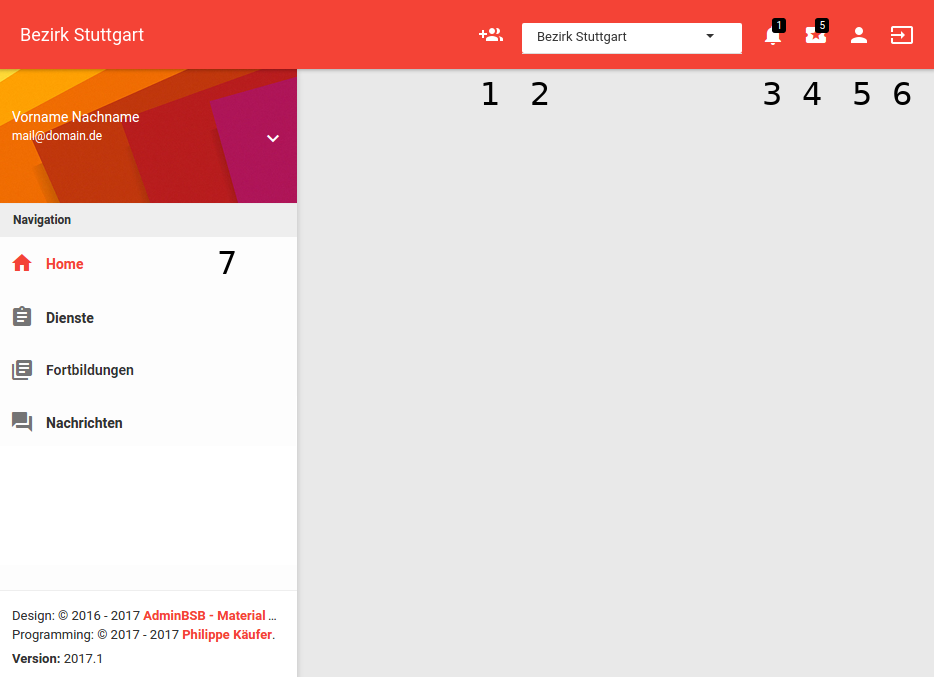
\includegraphics[width=14cm]{Bilder/view_menu.png}
 \end{addmargin} 
 \caption[Menü ansicht]{DLRG Dienstplan Menü ansicht}
 \label{fig:view_menu}
\end{figure}

\section{Registrieren für weitere Gliederungen}
\label{sec:menu_applyclient}
Ist ein Benutzer in mehreren Gliederungen tätig, kann er über den Menüpunkt eine Zuordnung zu weiteren Gliederungen beantragen. Die Administratoren der beantragten Gliederung müssen den Antrag bestätigen bevor dem Benutzer Zugriff gewährt wird.

\noindent (Abbildung \ref{fig:view_menu} \textit{\nameref{fig:view_menu}}, Markierung \textit{1})

\section{Wechseln der Gliederungen}
\label{sec:menu_changeclient}
Ist ein Benutzer mehreren Gliederungen zugeordnet, wird eine Dropdown-Liste angezeigt welches ein Wechsel der Ansicht zwischen den Gliederungen ermöglicht. Bei einem Login wird automatisch die zuletzt verwendete Gliederung geladen.

\noindent (Abbildung \ref{fig:view_menu} \textit{\nameref{fig:view_menu}}, Markierung \textit{2})

\section{Zugeteilte Dienste}
\label{sec:menu_approvedservice}
Darstellung als Schnellübersicht der bestätigten Dienste für den jeweiligen Benutzer.

\noindent (Abbildung \ref{fig:view_menu} \textit{\nameref{fig:view_menu}}, Markierung \textit{3})

\section{Eigene Qualifikationen}
\label{sec:menu_qualification}
Darstellung als Schnellübersicht der zugeteilten Qualifikationen für den jeweiligen Benutzer.

\noindent (Abbildung \ref{fig:view_menu} \textit{\nameref{fig:view_menu}}, Markierung \textit{4})

\section{Profil}
\label{sec:menu_profile}
Schnellzugriff auf das Benutzerprofil.

\noindent (Abbildung \ref{fig:view_menu} \textit{\nameref{fig:view_menu}}, Markierung \textit{5})

\vspace*{5mm} \noindent Im Profil kann ein Benutzer seine Daten ändern und auf dem Aktuellsten Stand halten. Wenn die Eingabe des Passwortes leer bleibt wird dieses nicht geändert. Beim erstmaligen Login empfiehlt es sich hier die Handynummer zu hinterlegen.  

\section{Logout}
\label{sec:menu_logout}
Über den Menüpunkt wird der Benutzer abgemeldet.

\noindent (Abbildung \ref{fig:view_menu} \textit{\nameref{fig:view_menu}}, Markierung \textit{6})

\section{Navigation}
\label{sec:menu_navigation}
Aufgrund einer niedrigen Auflösung oder kleineren Displaygröße wird bei manchen Geräten das Menü auf der Linken Seite \noindent (Abbildung \ref{fig:view_menu} \textit{\nameref{fig:view_menu}}, Markierung \textit{7}) nicht dargestellt. Das Menü kann dort über die links oben dargestellten drei Striche ein bzw. ausgeblendet werden.

\noindent Die Navigation enthält bei einem Benutzer folgende Einträge: 
\begin{itemize}
\item \nameref{cha:dashboard} (Kapitel: \ref{cha:dashboard})
\item \nameref{cha:dienste} (Kapitel: \ref{cha:dienste})
\item \nameref{cha:fortbildungen} (Kapitel: \ref{cha:fortbildungen}) \textit{Nur verfügbar, wenn diese für die jeweilige Gliederung freigeschaltet ist.}
\item \nameref{cha:nachrichten} (Kapitel: \ref{cha:nachrichten})

\end{itemize}
\include{Inhalt/qualification}
\chapter{Dashboard}
\label{cha:dashboard}

Das Dashboard bietet Überblicke und Statistiken. Ist ein Benutzer mehreren Gliederungen zugewiesen, wird auf dem Dashboard nur Inhalte der aktuell ausgewählten Gliederung dargestellt.

\begin{itemize}
\item Geleistete Dienste: Summe der Dienste aus der aktueller Saison, bei welchem der Benutzer eine Position übernommen hatte.
\item Total Geleistete Dienste: Summe der Positionen welche in der aktuellen Saison von allen geleistet wurde.
\item Noch nicht besetzte Dienste: Summe der zukünftig noch nicht besetzten Positionen. Hier werden nur Positionen welche für eine Mindestbesatzung relevant sind aufgezählt.
\item Hall of Fame: Benutzer mit den am meisten geleisteten Diensten der aktuellen Saison. 
\end{itemize}

\noindent Darunter sind News (Kapitel \ref{cha:nachrichten}) wie auch neue Infos zu finden. Diese werden meist ebenfalls per E-Mail den Benutzern zugestellt.

\begin{figure}[h]
 \begin{addmargin}{-0.2\linewidth}
   \centering 
   \includegraphics[width=20cm]{Bilder/view_overview.png}
 \end{addmargin} 
 \caption[Dashboard ansicht]{Dienstplan Dashboard ansicht}
 \label{fig:view_overview}
\end{figure}
\chapter{Dienste}
\label{cha:dienste}
Die Dienstübersicht zeigt alle zukünftigen Dienste absteigend sortiert nach Datum. Jeder Dienst wird als Block klar getrennt und übersichtlich dargestellt. In Abbildung \ref{fig:view_service} \textit{\nameref{fig:view_service}} ist ein einzelner Dienst exemplarisch abgebildet.

\begin{figure}[h]
 \begin{addmargin}{-0.2\linewidth}
   \centering 
   \includegraphics[width=20cm]{Bilder/view_service.png}
 \end{addmargin} 
 \caption[Dienste Übersicht]{Dienstplan Dienste Übersicht}
 \label{fig:view_service}
\end{figure}

\noindent Jeder Dienst ist mit Tag und Datum beschriftet. Darunter kann eine Bemerkung bzw. Beschreibung hinterlegt sein. Die einzelnen Positionen des Dienstes werden als Tabelle dargestellt. Positionen welche für eine Mindestbesatzung notwendig sind, werden unterstrichen dargestellt.
\noindent Dem Benutzer kann eine Position in fünf verschiedenen Ansichten präsentiert werden mit welchen er zum teil Interagieren kann.
Diese sind in der folgenden Tabelle aufgezeigt. Beispiele beziehen sich immer auf die Abbildung \ref{fig:view_service} \textit{\nameref{fig:view_service}}

\begin{itemize}
\item Melden (bsp. Position 4): Diese Position ist noch nicht zugeteilt. Der Benutzer kann sich hierzu melden.
\item Melden deaktiviert (bsp. Position 1): Diese Position ist noch nicht zugeteilt. Der Benutzer hat aber nicht die entsprechende Qualifikation und kann sich somit für die Position nicht melden.
\item Position bestätigt (bsp. Position 2): Die Position ist bereits zugeteilt.
\item Position bestätigt (bsp. Position 3): Diese Position ist an den Benutzer zugeordnet. Alle zugeordneten Positionen des eigenen Benutzers werden zur besseren Übersicht hellgrün dargestellt.
\item Für Position gemeldet, noch nicht bestätigt (bsp. Position 5): Für diese Position hat der Benutzer sich bereits gemeldet. Solange dies durch die Administratoren noch nicht bestätigt ist, kann die Meldung zurück gezogen werden.
\end{itemize}

\noindent Die in den orangenen Kästen dargestellten Zahlen stehen für die Anzahl an bereits gemeldeten Benutzern für diese Position. Ein Benutzer kann sich für beliebig viele Positionen eines Dienstes melden. Ebenso können beliebig viele Benutzer sich für eine Position melden. Durch die Administratoren wird nur einer Benutzer für eine Position bestätigt.

\noindent Positionen können Kommentare beinhalten (bsp. Position 1). Mit Kommentaren können geteilte Positionen (Position 1 nur bis 14 Uhr) realisiert werden. Des weiteren können mit Kommentaren auch auf Besonderheiten zu dieser Position hingewiesen werden.


\section{Mobile Ansicht}
\label{sec:dienste_mobile}
Die GUI auf Mobilgeräten, wie \zB Smartphones oder Tablets, weicht von der Desktopversion leicht ab. Die einzelnen Dienste sind eingeklappt und können mit einem Tippen auf den kleinen Pfeil oder das Datum ausgeklappt werden (\ref{fig:view_service_mobile_close} \textit{\nameref{fig:view_service_mobile_close}}). 


\begin{figure}[h]
 \begin{addmargin}{-0.2\linewidth}
   \centering 
   \includegraphics[width=20cm]{Bilder/view_service_mobile_close.png}
 \end{addmargin} 
 \caption[Dienste Übersicht Mobil]{Dienstplan Dienste Übersicht Mobil eingeklappt}
 \label{fig:view_service_mobile_close}
\end{figure}


\noindent Die rot hinterlegte Zahl zwischen dem kleinen Pfeil und dem Datum gibt die Anzahl der noch nicht zugewiesenen Positionen eines Dienstes an. Die Berechnung stützt sich hierbei lediglich auf Positionen welche für eine Mindestbesatzung relevant sind. In Abbildung \ref{fig:view_service_mobile} \textit{\nameref{fig:view_service_mobile}} ist die Zahl 6 zu sehen da wie in der ausgeklappten Ansicht zu sehen ist, 6 Positionen noch nicht zugewiesen wurden.

\begin{figure}[h]
 \begin{addmargin}{-0.2\linewidth}
   \centering 
   \includegraphics[width=20cm]{Bilder/view_service_mobile.png}
 \end{addmargin} 
 \caption[Dienste Übersicht Mobil Ausgeklappt]{Dienstplan Dienste Übersicht Mobil ausgeklappt}
 \label{fig:view_service_mobile}
\end{figure}
\chapter{Fortbildungen}
\label{cha:fortbildungen}
Die Fortbildungsübersicht zeigt alle zukünftigen Fortbildungen absteigend sortiert nach Datum. Jede Fortbildung wird als Block klar getrennt und übersichtlich dargestellt. In Abbildung \ref{fig:view_training} \textit{\nameref{fig:view_training}} ist eine einzelne Fortbildung exemplarisch abgebildet.

\begin{figure}[h]
 \begin{addmargin}{-0.2\linewidth}
   \centering 
   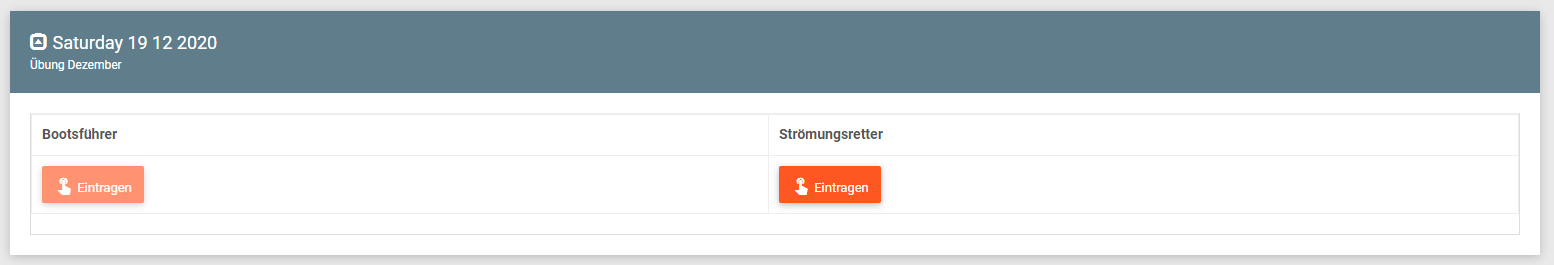
\includegraphics[width=20cm]{Bilder/view_training.png}
 \end{addmargin} 
 \caption[Fortbildungen Übersicht]{DLRG Dienstplan Fortbildung Übersicht}
 \label{fig:view_training}
\end{figure}

\noindent Jede Fortbildung ist mit Tag und Datum beschriftet. Darunter wird der Titel hinterlegt. Die einzelnen Positionen der Fortbildung werden als Tabelle dargestellt. Jeder Position können, wenn die entsprechende Qualifikation vorliegt, beliebig viele Helfer zugewiesen werden.
\noindent Dem Benutzer kann eine Position in drei verschiedenen Ansichten präsentiert werden mit welchen er zum teil Interagieren kann.
Diese sind in der folgenden Tabelle aufgezeigt.

\begin{itemize}
\item Melden: Diese Position ist noch nicht zugeteilt und die entsprechende Qualifikation liegt vor. Der Benutzer kann sich hierzu melden.
\item Melden deaktiviert: Diese Position ist noch nicht zugeteilt. Der Benutzer hat aber nicht die entsprechende Qualifikation und kann sich somit für die Position nicht melden.
\item Meldung zurückziehen: Nach einer Meldung für eine Position kann dies unmittelbar danach wieder zurückgezogen werden.
\end{itemize}

\noindent Positionen können Kommentare beinhalten. Mit Kommentaren werden z.B. auf Besonderheiten zu dieser Position hingewiesen.


\section{Mobile Ansicht}
\label{sec:training_mobile}
Die GUI auf Mobilgeräten, wie \zB Smartphones oder Tablets, weicht von der Desktopversion leicht ab. Die einzelnen Fortbildungen sind eingeklappt und können mit einem Tippen auf den kleinen Pfeil oder das Datum ausgeklappt werden (\ref{fig:view_training_mobile_close} \textit{\nameref{fig:view_training_mobile_close}}). 


\begin{figure}[h]
 \begin{addmargin}{-0.2\linewidth}
   \centering 
   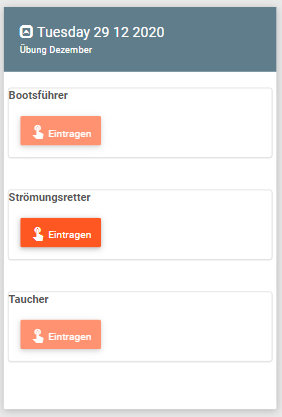
\includegraphics[width=8cm]{Bilder/view_training_mobile.png}
 \end{addmargin} 
 \caption[Fortbildungen Übersicht Mobil]{DLRG Dienstplan Fortbildung Übersicht Mobil}
 \label{fig:view_training_mobile_close}
\end{figure}
\chapter{Nachrichten}
\label{cha:nachrichten}

In dem Menüpunkt Nachrichten werden alle Nachrichten aufgelistet. Mithilfe von Nachrichten wird über aktuelle Ereignisse informiert. Die Nachrichten werden auch über den E-Mail Verteiler versendet.

\begin{figure}[h]
 \begin{addmargin}{-0.2\linewidth}
   \centering 
   \includegraphics[width=15cm]{Bilder/view_news.png}
 \end{addmargin} 
 \caption[Nachrichten]{Dienstplan Nachrichten}
 \label{fig:view_news}
\end{figure}
\chapter{Urlaub und Abwesenheit}
\label{cha:holidays}

Die Abwesenheiten von Helfenden kann auf zwei Arten im Portal hinterlegt werden:
\begin{enumerate}
	\item Urlaub oder Abwesenheit über einen Zeitraum. Hierfür muss über das Menü  die Seite \glqq Abwesenheit\grqq{} aufgerufen werden welche die Möglichkeit bietet alle aktuellen und zukünftigen Abwesenheiten zu bearbeiten oder neue anzulegen.
	
	\begin{figure}[h]
		\begin{addmargin}{-0.2\linewidth}
			\centering 
			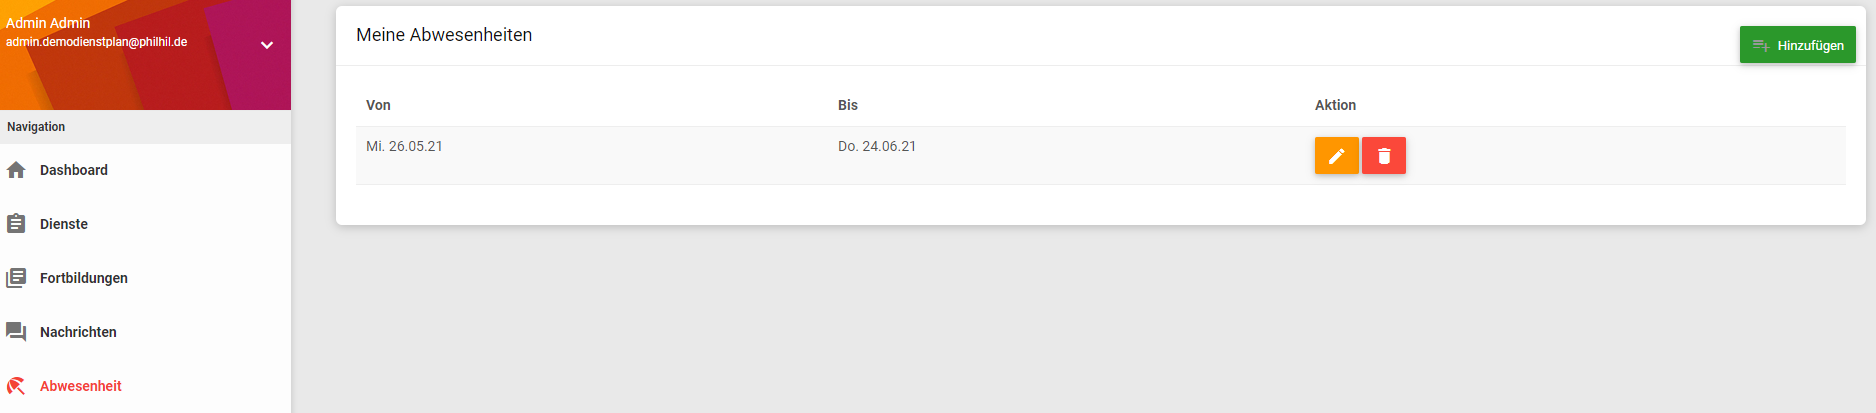
\includegraphics[width=15cm]{Bilder/view_holidays.png}
		\end{addmargin} 
		\caption[Urlaub und Abwesenheit]{Übersicht Abwesenheiten}
		\label{fig:view_holidays}
	\end{figure}
	
	\item Abwesenheit oder nicht Verfügbarkeit für einen einzelnen Dienst bzw. Tag. Für jeden Dienst oder Fortbildung kann rechts oben über die drei kleinen Punkte \glqq Keine Zeit\grqq{} gewählt werden. Dies erstellt automatisch einen Eintrag in den Abwesenheiten mit dem Datum des jeweiligen Dienstes.
	
	\begin{figure}[h]
		\begin{addmargin}{-0.2\linewidth}
			\centering 
			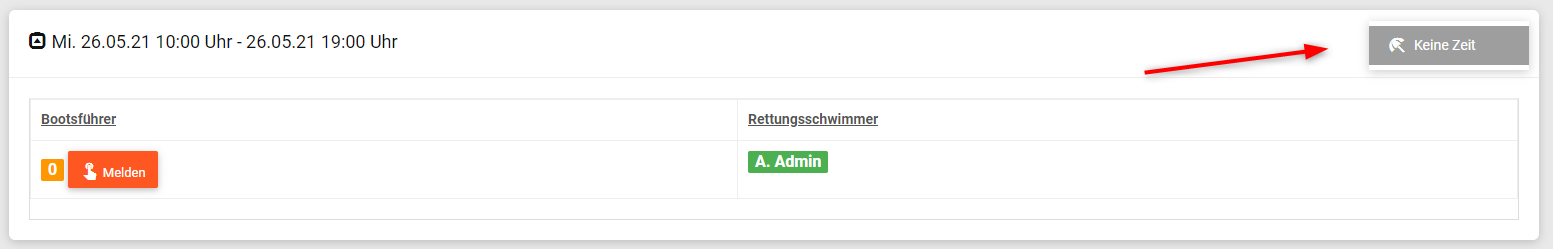
\includegraphics[width=15cm]{Bilder/view_service_holiday.png}
		\end{addmargin} 
		\caption[Abwesenheit]{Nicht verfügbar für einen Dienst / Tag}
		\label{fig:view_service_holiday}
	\end{figure}
\end{enumerate}


Alle Dienste und Fortbildungen, welche in einem Abwesenheits-Zeitraum liegen, werden in der jeweiligen Übersicht grau dargestellt. Die Dienstplan-Verwalter sehen ebenfalls, ob ein User im Urlaub ist. Der User kann sich trotzdem jederzeit für einen Dienst melden. 
\chapter{Kalender}
\label{cha:calendar}

Der Kalender gibt neben den Diensten und Fortbildungen vor allem über weitere Veranstaltungen eine Übersicht. Diese Veranstaltunen können von Administratoren und Fortbildungsverwaltenden dort hinterlegt werden.

Die verschiedenen Termin-Quellen können anhand der Farben unterschieden werden:
\begin{itemize}
    \item[\textbf{Rot:}] Dienst wo der Nutzer selbst eine Position besetzt.
	\item[\textbf{Grau:}] Dienst ohne eigene Beteiligung.
	\item[\textbf{Blaugrau:}] Training.
	\item[\textbf{Blau:}] Sonstiger Termin welcher manuell im Kalender angelegt wurde. Verantwortliche werden in klammern angezeigt.
\end{itemize}
\chapter{Prozesse}
\label{cha:prozesse}
In diesem Kapitel werden ausgewählte Standartprozesse zur Übersicht und späteren Orientierung der Benutzer definiert.

\section{Benutzer registrieren}
\label{sec:process_register}
Jeder Helfer benötigt einen eigenen Benutzeraccount. Dieser kann auf der Startseite unter \glqq Registrieren\grqq ~angelegt werden. Der Benutzer muss zunächst durch einen Administrator der Gliederung freigeschaltet werden. Der Benutzer wird via E-Mail über die Freischaltung automatisch informiert. Nach dem ein Benutzer Freigeschaltet wurde, wird der Administrator die entsprechenden Qualifikationen zuweisen. Wenn nicht alle bzw. die entsprechenden Qualifikationen zugewiesen wurden, sollten die Administratoren der Gliederung darauf aufmerksam gemacht werden.

\noindent \textit{Es ist möglich die selbe E-Mail Adresse wie bei Facebook zu verwenden. Hierdurch kann später das \glqq oneclick\grqq ~Login verfahren verwendet werden.}

\section{Dienst melden}
\label{sec:process_position_apply}
Für das Melden zu einem Dienst muss lediglich der entsprechende Tag gesucht werden. Bei Positionen mit entsprechender Voraussetzung an Qualifikationen kann der Benutzer sich direkt melden.

\noindent \textit{Ein Benutzer sollte sich bei einem Dienst zu mehreren Positionen melden. Die Administratoren werden nur einen bestätigen und haben somit mehr Flexibilität beim Besetzen der Dienste.}

\section{Dienst Aufteilen}
\label{sec:process_service_split}
Es ist möglich einzelne Dienste bzw. dessen Positionen in zwei Schichten aufzuteilen. Bereits geteilte Dienste sind an einem Kommentar der Position zu erkennen. Ist ein Dienst der geleistet werden will nicht aufteilt, werden die Administratoren durch einem freundlichen Hinweis per E-Mail dies einrichten.

\section{Dienst Absagen}
\label{sec:process_service_cancel}
Sollte ein Benutzer einen bereits gemeldeten Dienst absagen müssen, kann er dies, wenn noch nicht bestätigt, über \glqq Meldung zurückziehen\grqq ~(siehe Kapitel \ref{cha:dienste} \nameref{cha:dienste}) selber durchführen. Ist der Dienst bereits bestätigt, muss mit den Administratoren Kontakt aufgenommen werden.

\section{Fortbildung melden}
\label{sec:process_training_apply}
\textit{{\small Diese Funktion ist nicht bei allen Gliederungen aktiv.}}
Bei den Fortbildungen kann der Benutzer sich direkt für eine Position, bei welcher die entsprechende Voraussetzung an Qualifikationen vorliegen, melden.

\section{Für weitere Gliederung registrieren}
\label{sec:process_apply_client}
Benutzer können oben über das Schnellzugriff-Menü (\ref{sec:menu_applyclient} \nameref{sec:menu_applyclient}) eine Zuordnung zu weiteren Gliederungen beantragen. Der Benutzer muss durch einen Administrator der entsprechenden Gliederung freigeschaltet werden. Mit einer E-Mail wird der Benutzer über die Freischaltung informiert. Nach der Freischaltung, wird der Administrator die entsprechenden Qualifikationen zuweisen. Wenn nicht alle bzw. die entsprechenden Qualifikationen zugewiesen wurden, sollten die Administratoren der Gliederung darauf aufmerksam gemacht werden.
\chapter{Administrator}
\label{cha:administrator}
In diesem Kapitel wird die Sicht eines Administrators beleuchtet und dessen spezielle Berechtigungen und Aufgaben dargelegt.

\vspace*{5mm} \noindent Die Rolle des Administrators wird in Verbindung zu Gliederungen gesetzt. Ein Benutzer kann also Administrator von einer oder mehreren Gliederungen sein. Eine Gliederung muss durch mindestens einen, kann aber durch mehrere Benutzer administriert werden.

\vspace*{5mm} \noindent Die Navigation ist zusätzlich zu den Funktionen eines Benutzers um folgende Einträge erweitert: 
\begin{itemize}
	\item Benutzer (Kapitel: \ref{sec:admin_benutzerverwaltung})
	\item Dienste bestätigen
	\item Dienst anlegen (Kapitel: \ref{sec:admin_service})
	\item Fortbildung anlegen (Kapitel: \ref{sec:admin_training})
    \item Kalendereintrag anlegen
	\item Nachricht erstellen (Kapitel: \ref{sec:admin_news})
	\item Abfragen (Kapitel: \ref{sec:admin_survey})
	\item Qualifikationen (Kapitel: \ref{sec:admin_qualifikationsverwaltung})
	\item Client (Kapitel: \ref{sec:admin_gliederungsverwaltung})
\end{itemize}

\section{Gliederungsverwaltung}
\label{sec:admin_gliederungsverwaltung}
Über den für Administratoren eingeblendeten Menüpunkt \noindent (Abbildung \ref{fig:view_client} \textit{\nameref{fig:view_client}}, Markierung \textit{1}, rechts oben) kann die Eigenschaften-Seite einer Gliederung aufgerufen werden um diese zu konfigurieren.

\begin{itemize}
	\item[\textbf{Name:}] Name der Gliederung. Dieser wird oben links, in der Gliederungsauswahl wie auch bei der Registrierung verwendet.
	\item[\textbf{Start der Saison:}] Gibt den Saison-Start an. Statistiken und Graphen welche nur für eine Saison Daten aggregieren, werden zu dem Datum zurückgesetzt.
	\item[\textbf{Dienstbeginn:}] Angabe wann ein Dienst standardmäßig beginnt. Dies dient einer schnelleren Administration und wirkt sich als vorausgefüllte Formularfelder aus.
	\item[\textbf{Dienstende:}] Angabe wann ein Dienst standardmäßig endet. Dies dient einer schnelleren Administration und wirkt sich als vorausgefüllte Formularfelder aus.
	\item[\textbf{Automatismen:}]
	\begin{itemize}
		\item Wöchentliches versenden des Wachplans: Wenn dies ausgewählt ist, wird jeden Montag der Wachplan unter folgenden Bedingungen versendet: Es existiert in den Kommenden zwei Wochen mindestens ein Dienst. 
		
		\noindent Die Mail wird den Wachplan für die nächsten zwei Monate beinhalten.
	\end{itemize}
	\item[\textbf{Mailingliste:}]
	\begin{itemize}
		\item Checkbox: Wenn dies ausgewählt ist, werden E-Mails nicht an jeden Nutzer einzeln sondern an eine Mailingliste versendet. Hierdurch können auch Personen außerhalb des Dienstplan-Portals Informationen wie z.B. Nachrichten oder den wöchentlichen Dienstplan erhalten.
		\item Mailingliste E-Mail: Definiert an welche E-Mail Adresse (Mailingliste) gesendet werden soll, wenn die Checkbox gesetzt ist.
	\end{itemize}
	\item[\textbf{Absender:}]
	\begin{itemize}
		\item Absender Name: Name welcher als Absender von ausgehenden Mails angezeigt wird.
		\item Antworten an E-Mail Adresse: E-Mail Adresse von welcher E-Mails versendet werden. Hier sollte eine ...@gliederung.dlrg.de Adresse hinterlegt sein.
	\end{itemize}
	\item[\textbf{Admin Zuteilung:}]
	\begin{itemize}
		\item Hier können der Gliederung weitere Administratoren zugeordnet werden. 
	\end{itemize}
	\item[\textbf{Fortbildung Editor:}]
	\begin{itemize}
		\item Die Berechtigung Fortbildung Editor ermöglicht die Verwaltung von Fortbildungen expliziten Benutzern zu übertragen welche keine Administrationsrechte inne haben.
	\end{itemize}
\end{itemize}

\begin{figure}[h]
	\begin{addmargin}{-0.2\linewidth}
		\centering 
		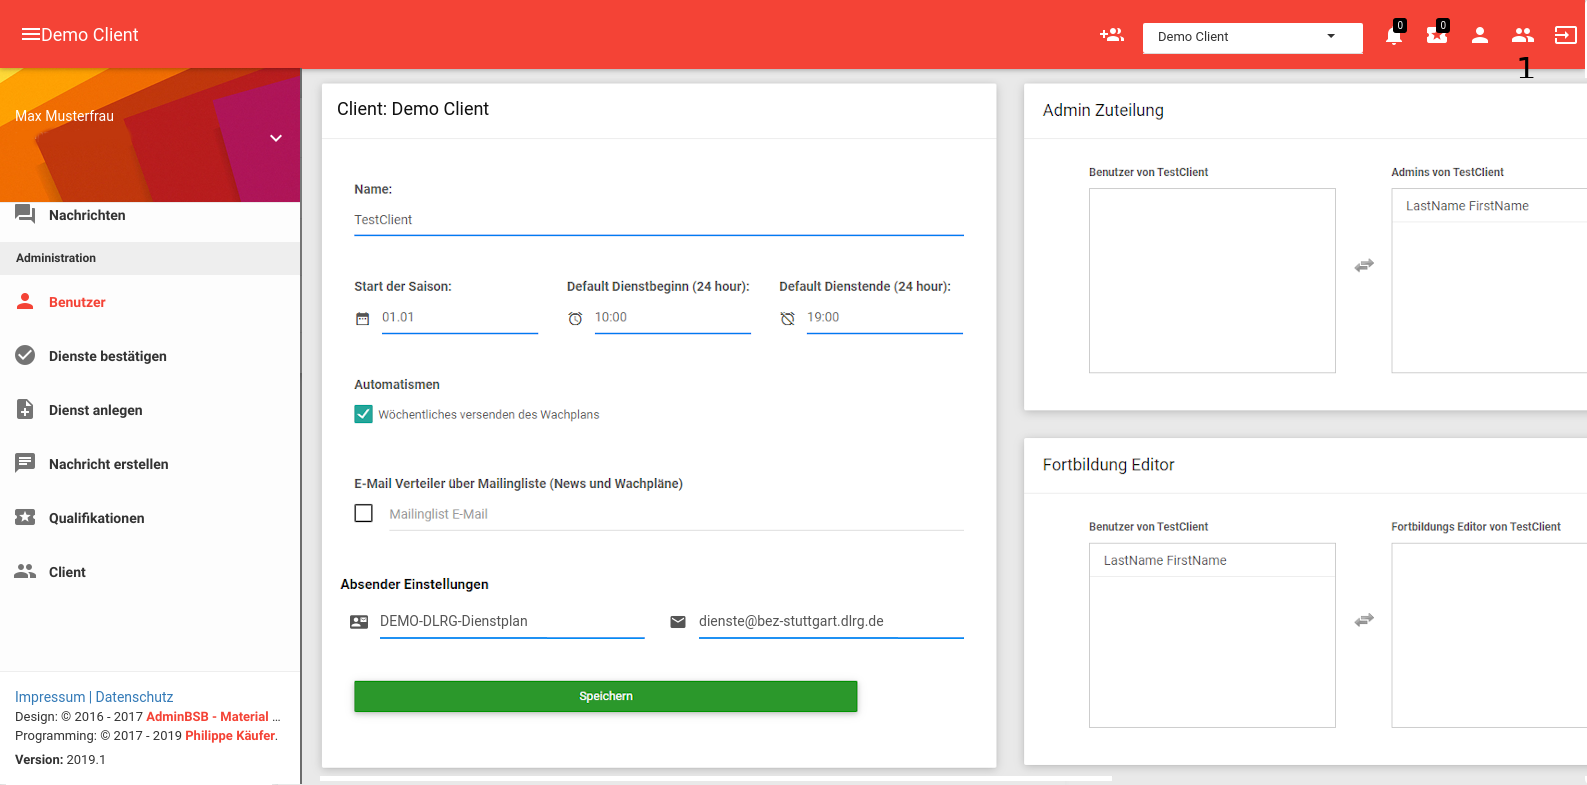
\includegraphics[width=20cm]{Bilder/view_admin.png}
	\end{addmargin} 
	\caption[Gliederungsverwaltung]{Dienstplan Gliederungsverwaltung}
	\label{fig:view_client}
\end{figure}

\section{Benutzerverwaltung}
\label{sec:admin_benutzerverwaltung}
In dem Menüpunkt Benutzer werden alle Benutzer der aktuellen Gliederung tabellarisch aufgelistet. Über diese Tabelle stehen drei Aktionen zu Verfügung:

\begin{table}[H]
	\centering
	\begin{tabular}{ll}
		\includegraphics[width=1.5cm]{Bilder/edit.png} & Editieren der Eigenschaften eines Benutzers. \\[10pt]
		\includegraphics[width=1.5cm]{Bilder/approve.png}	& Benutzer für die Gliederung freigeben. \\[10pt]
		\includegraphics[width=1.5cm]{Bilder/remove.png} & Die Zuordnung des Benutzer mit der aktuellen Gliederung löschen. \\
	\end{tabular}
	%\caption{Übersicht Icons und Funktionen Benutzerverwaltung}
	%\label{fig:admin_benutzerverwaltung}
\end{table}

\section{Qualifikationsverwaltung}
\label{sec:admin_qualifikationsverwaltung}
Qualifikationen stellen die zentrale Komponente um Benutzen die Berechtigung zu erteilen, Positionen zu besetzen. Hierfür werden zunächst Qualifikationen angelegt. Darauf aufbauend sind beim anlegen eines Dienstes den einzelnen Positionen basierend auf Qualifikationen zuzuordnen. Im Dienstplan können folgend nur Benutzer, welche diese Qualifikation zugewiesen bekommen haben, sich bei entsprechenden Positionen melden. Beispiel: Zunächst wird eine Qualifikation Sanitäter angelegt. Diese Qualifikation wird Benutzern über die \ref{sec:admin_benutzerverwaltung} \nameref{sec:admin_benutzerverwaltung} zugewiesen. Werden Dienste mit Positionen \glqq Sanitäter\grqq{} angelegt, können nur entsprechende Nutzer mit der Qualifikation \glqq Sanitäter\grqq{} sich für diese Position melden.

\vspace*{5mm} \noindent Das anlegen von Qualifikationen bedingt folgende Eingaben:

\begin{itemize}
	\item[\textbf{Name:}] Name der Qualifikation.
	\item[\textbf{Abkürzung:}] Abkürzung der Qualifikation. Diese Abkürzung wird verwendet, wenn der Name für Eingabefelder, Anzeigen oder Ausdrucke zu lang ist. Es wird empfohlen hier max. 5 Zeichen zu verwenden.
	\item[\textbf{Default:}] \glqq Soll die Qualifikation bei anlegen von einem Service automatisch erstellt werden?\grqq{} Ist die Checkbox markiert, werden beim erzeugen eines Dienstes automatisch Positionen mit dieser Qualifikation angelegt.
	\item[\textbf{Default Anzahl:}] Gibt die Anzahl der Positionen an, welche beim erzeugen von Diensten automatisch angelegt werden.
	\item[\textbf{Erforderlich:}] Ist eine Position bei Diensten zwingend erforderlich, kann diese markiert werden (ref.: \ref{sec:admin_service} \nameref{sec:admin_qualifikationsverwaltung}). Diese Checkbox gibt den Standartwert vor, wenn eine Position mit dieser Qualifikation automatisch oder manuell einem Dienst hinzugefügt wird.
\end{itemize}

\begin{lamp}[frametitle={Qualifikationen Benutzern zuweisen}]
	Über die Benutzerverwaltung können Qualifikationen den Benutzern zugewiesen werden. Die Zuweisung erfolgt getrennt für jede Gliederung/Mandant. Mit dem Zuweisen werden Benutzer automatisch via E-Mail über diese Aktion informiert.
\end{lamp}

\section{Dienstverwaltung}
\label{sec:admin_service}
Dienste bestehen aus mindestens einer und beliebig vielen Positionen. Über den Menüpunkt Dienste (Kapitel \ref{cha:dienste} \nameref{cha:dienste}) werden alle angelegten Dienste der aktuellen Saison angezeigt. Das Anlegen von Diensten unterliegt den Administratoren einer Gliederung und erfolgt unter dem Menüpunkt \glqq Dienst anlegen \grqq{}. Ein Dienst hat folgende Eigenschaften:

\begin{itemize}
	\item[\textbf{Datum:}] Datum des Dienstes.
	\item[\textbf{Freigabe:}] Wenn Personen sich auf eine Position melden, müssen diese erst von einem Administrator bestätigt werden.
	\item[\textbf{Bemerkung:}] Dieses Feld kann z.B. für dem Namen einer Veranstaltung o.ä. verwendet werden. Alternativ ist dieses leer zu lassen.
	\item[\textbf{Positionen:}] Es können beliebig viele Positionen mit folgenden Eigenschaften hinzugefügt werden:
	\begin{itemize}
		\item \textbf{Qualifikation:} Definiert die Qualifikation für diese Position.
		\item \textbf{Person:} Zugewiesene Person. Beim anlegen kann dies auf \glqq -- Bitte wählen -- \grqq{} gesetzt bleiben. Soll Direkt eine Person zugewiesen werden ist diese aus dem Dropdown zu wählen. Die Liste ist nach Nachnamen sortiert, auch wenn die Anzeige den ersten Buchstabe des Vornamens mit anzeigt. Personen mit passender Qualifikation sind grün hinterlegt. Grau hinterlegte Personen mit einem vorangestellten X haben sich zu der Dienstzeit als abwesend markiert. Personen welche Positionen neu zugeteilt wurden, werden via E-Mail automatisch darüber in Kenntnis gesetzt.
		\item \textbf{Kommentar:} Optionales Feld für z.B. Infos wenn eine Position eine extra Sonderaufgabe zugewiesen wird oder eine andere Dienstzeit aufweist.
		\item \textbf{Erforderlich:} Ist diese Position zwingend zu besetzten oder optional? Hat Auswirkung auf die Rote Zahl der freien Dienste in der Dienstauflistung (\ref{cha:dienste} \nameref{cha:dienste}) sowie auf die Statistiken.
	\end{itemize}
\end{itemize}
Melden sich Personen selbständig für Dienste bzw. deren Positionen, werden alle Admins via E-Mail darüber in Kenntnis gesetzt. Die Freigabe erfolgt über die Admins auf der Dienste Ansicht (ref.: \ref{cha:dienste} \nameref{cha:dienste}). Eine Freigabe löst wiederum eine automatische Benachrichtigung der betroffenen Person aus.

\section{Fortbildungsverwaltung}
\label{sec:admin_training}
\textit{{\small Um diese Funktion zu nutzen, muss das Modul Fortbildungen freigeschaltet sein.}}
Fortbildungen bestehen aus mindestens einer und beliebig vielen Positionen. Über den Menüpunkt Fortbildungen (Kapitel \ref{cha:fortbildungen} \nameref{cha:fortbildungen}) werden alle angelegten Fortbildungen der aktuellen Saison gezeigt. Das Anlegen von Fortbildungen unterliegt den Administratoren und Fortbildungs Editoren einer Gliederung und erfolgt unter dem Menüpunkt \glqq Fortbildung anlegen \grqq{}. Eine Fortbildung hat folgende Eigenschaften:

\begin{itemize}
	\item[\textbf{Datum von:}] Start Datum und Uhrzeit der Fortbildung.
	\item[\textbf{Datum von:}] End Datum und Uhrzeit der Fortbildung.
	\item[\textbf{Titel:}] Titel der Fortbildung welcher in der Auflistung Fortbildungen mit angezeigt wird.
	\item[\textbf{Text:}] Dieses Feld beschreibt die Fortbildung und wird in der Ankündigungs- E-Mail als Text verwendet.
	\item[\textbf{Ort:}] Beschreibt den Ort der Fortbildung. Wenn hier GPS Koordinaten eingetragen werden können die Fortbildungen in einer Späteren Version des Portals auf einer Karte dargestellt werden.
	\item[\textbf{E-Mail:}] Wenn hier ein Datum mit Zeit hinterlegt ist, wird je nach Einstellung der Gliederung, eine Ankündigungs- E-Mail an alle Nutzer oder an die Mailingliste versendet. Die E-Mail enthält Titel, Start- und End-Datum wie auch der Beschreibungstext.
	\item[\textbf{Positionen:}] Es können beliebig viele Positionen mit folgenden Eigenschaften hinzugefügt werden:
	\begin{itemize}
		\item \textbf{Qualifikation:} Definiert die Qualifikation für diese Position.
		\item \textbf{Kommentar:} Optionales Feld für z.B. Infos wenn eine Position eine extra Sonderaufgabe zugewiesen wird oder eine andere Dienstzeit aufweist.
		\item \textbf{Punkte:} Jeder Position können Fortbildungspunkte zugewiesen werden. Hiermit ist eine Fortbildungs-Übersicht möglich. Wird dieses Feature nicht aktiv genutzt, sollte der default wert 1 verwendet werden.
	\end{itemize}
\end{itemize}

\noindent Zuweisungen von Nutzern zu Fortbildungen:
Analog den Diensten (Kapitel \ref{cha:dienste} \nameref{cha:dienste}) kann sich jeder Nutzer selbst auf Positionen von Fortbildungen für welche die entsprechende Qualifikation vorliegt melden. Fortbildungs-Editoren und Administratoren können des weiteren unabhängig der Qualifikation Nutzer den Positionen zuteilen. Hierzu wird in der Ansicht Fortbildungen (Abbildung \ref{fig:view_training_admin} \textit{\nameref{fig:view_training_admin}}) ein Button bei jeder Position dargestellt. Über diesen Button wird die Helfer Zuteilung der jeweiligen Position geöffnet.

\begin{figure}[h]
	\begin{addmargin}{-0.2\linewidth}
		\centering 
		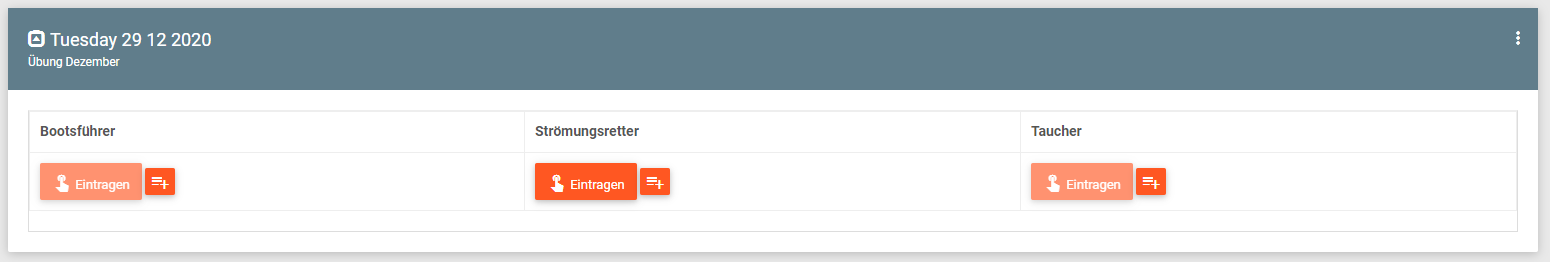
\includegraphics[width=20cm]{Bilder/view_training_admin.png}
	\end{addmargin} 
	\caption[Fortbildungen Admin Ansicht]{Dienstplan Fortbildungsansicht für Admin und Fortbildungs-Editor}
	\label{fig:view_training_admin}
\end{figure}
Über die Helfer Zuteilung (Abbildung \ref{fig:view_training_assign} \textit{\nameref{fig:view_training_assign}}) können Nutzer der Position zugeteilt werden. Die Spalte Qualifikation wird bei Nutzern welche die entsprechende Qualifikation der Position inne haben grün markiert. Zugeteilte Nutzer werden durch eine der Farbe Cyan markierte Zeile dargestellt. Mit Klick auf die Zeile werden Nutzer zugeteilt bzw. eine Zuteilung entfernt. Nutzer erhalten im Gegensatz zu Diensten keine E-Mail-Benachrichtigung hiervon.

\begin{figure}[h]
	\begin{addmargin}{-0.2\linewidth}
		\centering 
		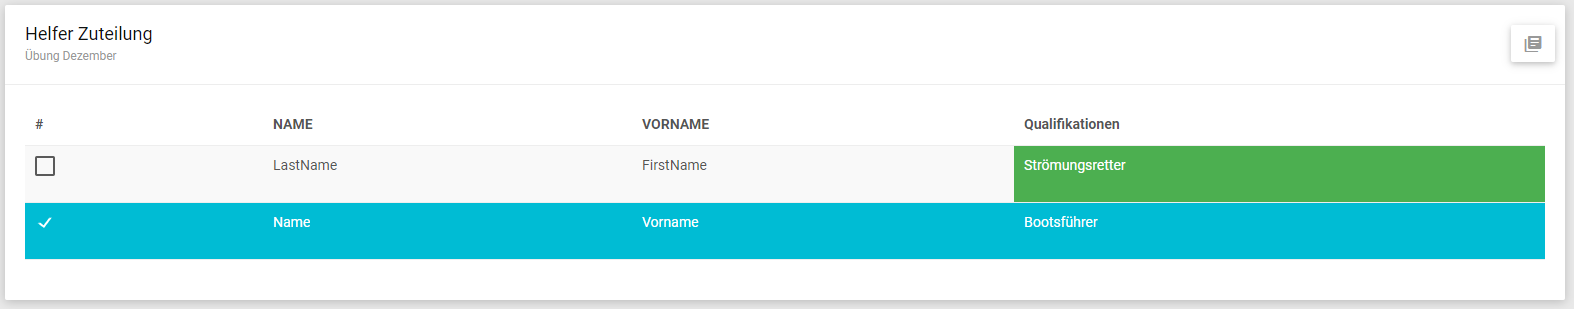
\includegraphics[width=20cm]{Bilder/view_training_assign.png}
	\end{addmargin} 
	\caption[Fortbildungs-Zuweisung]{Dienstplan Fortbildungs-Zuweisung}
	\label{fig:view_training_assign}
\end{figure}

\section{Abfragen und Bestätigungen}
\label{sec:admin_survey}
\textit{{\small Um diese Funktion zu nutzen, muss das Modul Abfragen und Bestätigungen freigeschaltet sein.}}

Mittels Abfragen werden in definierten Zeiträumen den Benutzern diese auf allen Seiten sehr präsent eingeblendet. Allgemein können diese für Umfragen oder Belehrung und Bestätigung sowie deren Rückmeldungen dokumentieren genutzt werden. Somit kann z.B. eine Durchführung von UVV Unterweisung oder Abfragen von aktuellen Kontaktdaten realisiert werden.
Benutzer können Abfragen drei mal verschieben bevor diese zwingend beantwortet werden müssen. Abfragen müssen je nach Eigenschaften von den Benutzern mit einem Passwort bestätigt werden, um der Abfrage einen offiziellen charakter zu verleihen.

Hier eine kurze Erläuterung zu den Besonderheiten der Eigenschaften von Abfragen:
\begin{description}
    \item[\textbf{Titel:}] Titel der Abfrage welcher kurz und knapp sein sollte, da dieser in einem kleinen Meldungsfeld den Nutzern angezeigt werden.
	\item[\textbf{Text:}] Text welcher Handlungsanweisungen an Nutzern gibt. Das Abstimmen oder zustimmen der Nutzer hängt von diesem Text ab.
	\item[\textbf{Von:}] Ab welchem Datum die Abfrage starten soll. Bei leerer eingabe wird die Abfrage sofort gestartet.
	\item[\textbf{Bis:}] Bis welchem Datum die Abfrage durchgeführt werden soll. Bei leerer eingabe wird die Abfrage für immer laufen. D.h. Neuregistrierung bekommen diese Abfragen beim ersten Login auch sofort angezeigt.
	\item[\textbf{Abfrage muss zugestimmt werden:}] Aktiviert: Nutzer haben nur die Möglichkeit zuzustimmen. Deaktiviert: Nutzer können Abfragen zustimmen oder ablehnen.
	\item[\textbf{Nutzer müssen Passwort zum zustimmen eingeben:}] Es kann nur mit dem eigenen Passwort zugestimmt oder abgelehnt werden.
	\item[\textbf{Nur für Nutzer mit Qualifikation::}] Abfragen werden nur Nutzern mit entsprechender Qualifikation angezeigt. Sollen mehrere Qualifikationen berücksichtigt werden, müssen mehrere Abfragen erstellt werden.
\end{description}

\section{Nachrichtenverwaltung}
\label{sec:admin_news}
Verfasste Nachrichten werden an alle Nutzer versendet. Je nach Einstellung der Gliederung wird eine E-Mail an die Mailingliste oder aber an jeden Benutzer einzeln versendet.
Nachrichten werden unter dem Menüpunkt \glqq Nachrichten\grqq{} Chronologisch aufgelistet. Zusätzlich wird die neueste Nachricht auf dem Dashboard (ref.:\ref{cha:dashboard} \nameref{cha:dashboard}) dargestellt.
\chapter{Module}
\label{cha:module}
Die Applikation ist in modularen Modulen untergliedert. Je nach Anforderung und Bedürfnis können einzelne Module für Gliederungen aktiviert werden.
Die aktuell aktiven Module werden den Administratoren der Gliederung unter der Gliederungsverwaltung \noindent (Abbildung \ref{fig:view_client} \textit{\nameref{fig:view_client}}, Markierung \textit{1}, rechts oben) aufgelistet\\

\noindent Die aktuell aktivierbaren Module sind folgend aufgelistet:

\begin{description}
	\item[Dienstplan:] Dies stellt das Kernmodul dar welches automatisch für jede Gliederung aktiv ist. Das Modul beinhaltet die Grundfunktionen wie Benutzerverwaltung, Qualifikationen, Nachrichten, E-Mail Versand wie auch die Dienstplanung selbst.

    \item[Abfragen und Bestätigungen:] Aktiviert das Verwalten von Abfragen und Bestätigungen dieser. Abfragen dienen zur Belehrung und Bestätigung und dokumentieren Rückmeldungen der Nutzer. Z.B. Durchführung von UVV Unterweisung oder Abfragen von aktuellen Kontaktdaten.

	\item[Fortbildungen:] Mit diesem Modul werden Fortbildungen verwaltet.
	In Abgrenzung zu Diensten können Positionen einer Fortbildung durch beliebig viele Benutzer besetzt werden. 
	Modul-Voraussetzungen: Dienstplan

    \item[Credits für Fortbildungen:] Aufbauend auf dem Modul Fortbildungen können Credits für einzelne Fortbildungspositionen verwaltet werden. Hiermit sind Fortbildungsübersichten über Saisons für jeden User in seinem Profil einsehbar.

    \item[Erweiterte Statistik:] Aktiviert das Modul Statistik welches die Möglichkeit der Auswertung von Zeiträumen sowie erweiterte Reports ermöglicht.

\end{description}

\chapter{Aussicht}
\label{cha:aussicht}
Das Dienstplan-Portal soll stetig weiterentwickelt und verbessert werden. Hierzu sind im allgemeinen Feedback und Vorschläge immer willkommen!

\vspace*{5mm} \noindent Fehler, Erweiterungen und Wünsche werden bei der Codeverwaltung mit geführt: \url{https://github.com/Philhil/DienstplanDLRG/issues}
Direkte Einflussnahme und Diskussion zu Verbesserungen kann dort geschehen oder über E-Mail.

\vspace*{5mm} \noindent Funktionen die in Zukunft folgen:

\begin{itemize}
\item Spezial Aufgaben: Es ist wünschenswert Spezialaufgaben wie z.B. Kochen für einen Dienst im Dienstplan-Portal festzulegen. 
\item Message Funktion innerhalb eines Dienstes: Für die vorab Kommunikation einer Dienst-Mannschaft ist es hilfreich dort eine direkte Kontaktmöglichkeit zu schaffen. Denkbar: Gruppenführer kann E-Mail versenden, Whatsapp Gruppe erstellen...
\item Kalender Funktion: Jeder Benutzer kann für sein Handy/Desktop Kalender den Dienstplan abbonieren. Bestätigte (und gemeldete?) Dienste würden so direkt im gewohnten Kalender vermerkt.
\item Hier könnte deine Idee stehen!
\end{itemize}

% ---------------------------- Literaturverzeichnis ----------------------------------------------

\begin{thebibliography}{999999}

%\bibitem {Buchtitel} Author: \emph{Buchtitel}, Erscheinungsort: Verlag, Jahr

\bibitem {Responsive_Webdesign} Wikipedia: \emph{Responsive Webdesign}, \url{https://de.wikipedia.org/wiki/Responsive_Webdesign}, 15 12 2017.

\bibitem {Facebook_Login} Facebook: \emph{Facebook Login für das Web mit dem JavaScript-SDK}, \url{https://developers.facebook.com/docs/facebook-login/web}, 28 12 2017.


\end{thebibliography}

% ------------------------------- Anhang ---------------------------------------------------------

\begin{appendix}
\clearpage
\pagenumbering{Roman}						% römische Seitenzahlen für Anhang
\end{appendix}


\end{document}